\documentclass{standalone}
\usepackage{tikz}
\usetikzlibrary{shapes}
\usetikzlibrary{positioning}
\usepackage{amsmath}


\begin{document}
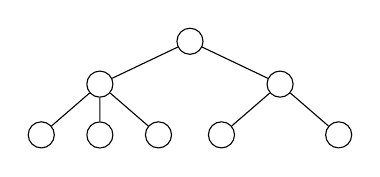
\begin{tikzpicture}[node distance=2cm]

    % \node(start)[startstop]{Start};
    \node(B1)[draw, circle, minimum size=0.2cm]{};
    \node(A1)[draw, circle, minimum size=0.2cm, above right=0.3cm and 0.9cm of B1]{};
    \node(F1)[draw, circle, minimum size=0.2cm, below left=0.4cm and 0.5cm of B1]{};
    \node(G1)[draw, circle, minimum size=0.2cm, below=0.3cm of B1]{};
    \node(H1)[draw, circle, minimum size=0.2cm, below right=0.4cm and 0.5cm of B1]{};

    \node(E1)[draw, circle, minimum size=0.2cm, below right=0.3cm and 0.9cm of A1]{};
    \node(I1)[draw, circle, minimum size=0.2cm, below left=0.4cm and 0.5cm of E1]{};
    \node(K1)[draw, circle, minimum size=0.2cm, below right=0.4cm and 0.5cm of E1]{};

    \draw (A1) -- (B1) -- (F1);
    \draw (H1) -- (B1) -- (G1);
    \draw (A1) -- (E1);
    \draw (K1) -- (E1) -- (I1);



\end{tikzpicture}
\end{document}
